\normaltrue \difficilefalse \tdifficilefalse
\correctionfalse
%\UPSTIidClasse{11} % 11 sup, 12 spé
%\newcommand{\UPSTIidClasse}{11}

\exer{Micromanipulateur $\star$ \label{C2:04:66}}
% CCP PSI 2009
\setcounter{question}{0}\UPSTIcompetence[2]{C2-04}
\index{Compétence C2-04}
\index{Correcteur}
\index{Correcteur proportionnel intégral}
\index{Micromanipulateur}


\ifcorrection
\else
\marginnote{\textbf{Pas de corrigé pour cet exercice.}}
\fi


\ifprof
\else
Pour élever la température à c\oe{}ur du moteur, on alimente en tension tous les bobinages du moteur par l'intermédiaure d'un comparateur et d'un amplificateur. Cet ensemble élabore une tension, dépendant de la teion de consigne $u_c(t)$, provenant d'un dispositif non étudié ici, et de la tension $u_m(t)$ fournie par un capteur de température situé dans le stator du moteur. 

\begin{center}
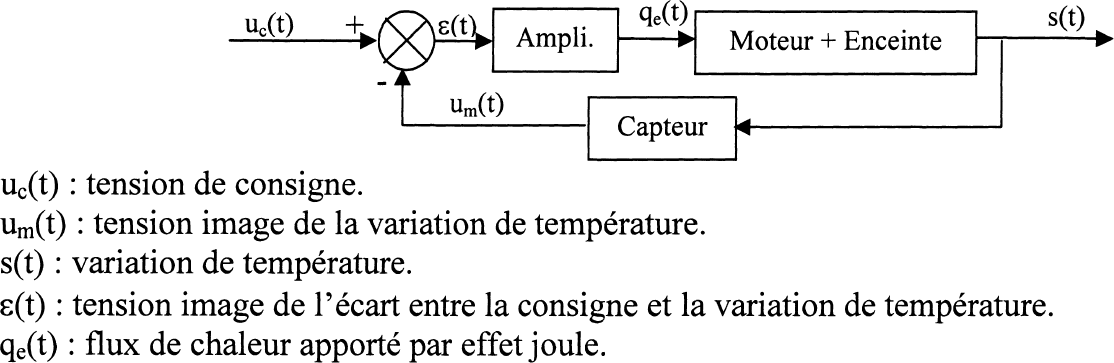
\includegraphics[width=\linewidth]{66_01}
\end{center}


L'ensemble \{Moteur + enceinte \} est modélisé par un premier ordre de fonction de transfert $H(p)=\dfrac{H_0}{1+\tau p}$
avec $H_0 = \SI{0}{\degres C.W^{-1}}$ et $\tau=\SI{200}{s}$?

Le capteur es tmodélisé par un système de fonction de transfert $\beta \exp^{-T_r p}$ avec $\beta = \dfrac{5}{200}\si{V.\degres C^{-1}}$ et $T_r = \SI{20}{s}$.

L'amplificateur est modélisé par un gain pur $A= \SI{400}{W.V^{-1}}$

Le cahier des charges est le suivant. 

\begin{center}
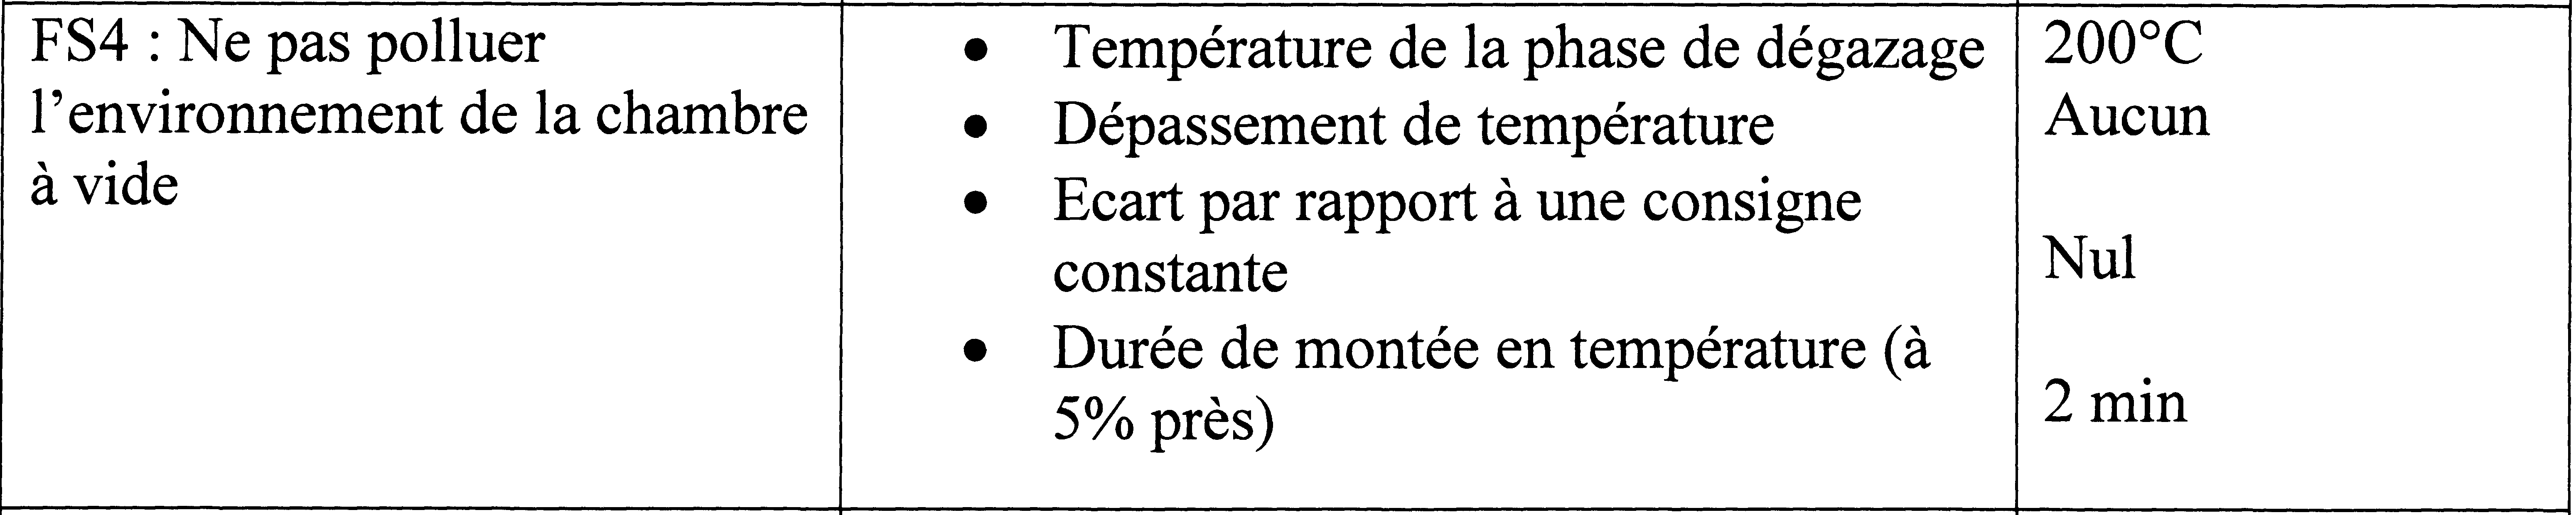
\includegraphics[width=\linewidth]{66_02}
\end{center}
\fi

\question{Expliquez en quelques lignes pourquoi le retard engendé par le capteur risque de rendre le système non conforme au cahier des charges.}
\ifprof
\else 
\fi


\ifprof
\else 
Pour supprimer l'inflience du retard, on choisit d'unsatller un correcteur en série juste avant l'amplificateur, comme indiqué sur le schéma-blocs suivant. 

\begin{center}
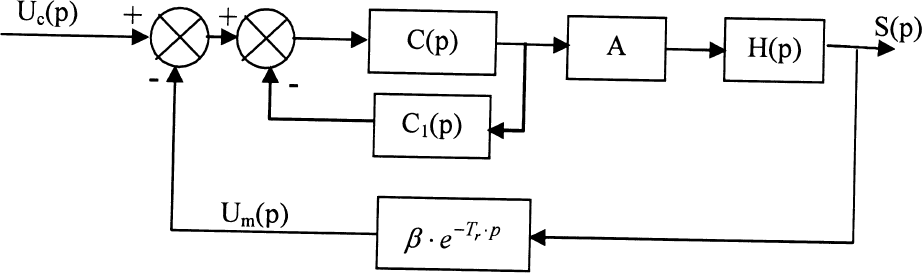
\includegraphics[width=\linewidth]{66_03}
\end{center}
\fi

\question{Déterminer l'expression littérale de la fonction de transfert en boucle fermée du système ainsi corrigé en fonction de $H(p)$, $A$, $C(p)$, $C_1(p)$, $\beta$ et $T_r$.}
\ifprof
\else 
\fi

\question{Déterminer l'expression de $C_1(p)$ en fonction de $H(p)$, $A$, $\beta$ et $T_r$, pour que le système ait un comportement équivalent au système sans retard suivant.}
\ifprof
\else 
\fi

\ifprof
\else 

\begin{center}
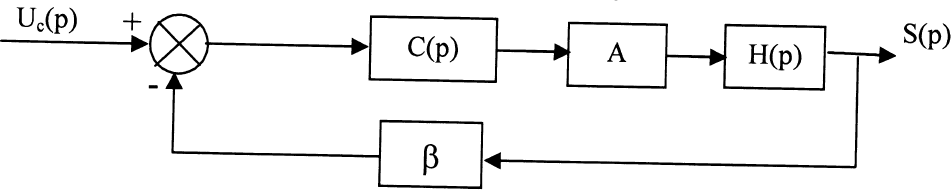
\includegraphics[width=\linewidth]{66_04}
\end{center}

Grâce au correcteur $C(p)$ choisi précédemment, le retard n'a plus d'influence sur la commande du système. 

On choisit comme fonction de transfert de la seconde partie du ocrrecteur $C(p)=K_i \dfrac{1+T_i p}{T_i p}$. 
\fi

\question{Justifier le choix de $C(p)$ en vous appuyant sur les exigences du cahier des charges.}
\ifprof
\else 
\fi

\question{Déteminer l'expression de la fonction de transfert en boucle fermée $F(p)=\dfrac{S(p)}{U_c(p)}$ du système en fonction de $K_i$ et $T_i$.}
\ifprof
\else 
\fi

\question{Calculer la valeur de $T_i$ pour que le système se comporte comme un premier ordre.}
\ifprof
\else 
\fi

\question{Calculer la valeur de $K_i$ pour que le temps de montée en température soit compatible avec les données du cahier des charges.}
\ifprof
\else 
\fi


\ifprof
\else

\noindent\footnotesize
 \fbox{\parbox{.9\linewidth}{
Éléments de corrigé : 
\begin{enumerate}
\item .
\item $H_{\text{BF corrigee}} = \dfrac{AHC}{1+CC_1+AHC\beta \exp^{-T_r p}}$.
\item $C_1=AH\beta \left( 1- \exp^{-T_r p}\right)$.
\item .
\item $F(p)=\dfrac{AH_0K_i\left(1+T_i p\right)}{\left(1+\tau p\right)T_i p+A\beta H_0K_i \left(1+T_i p\right)}$.
\item $T_i = \tau$.
\item $K_i  = \dfrac{\tau }{40 A\beta H_0} = 25$.
\end{enumerate}}}
\normalsize

\begin{flushright}
\footnotesize{Corrigé  voir \ref{C2:04:66}.}
\end{flushright}%
\fi